\begin{figure}[htbp]
  \centering
  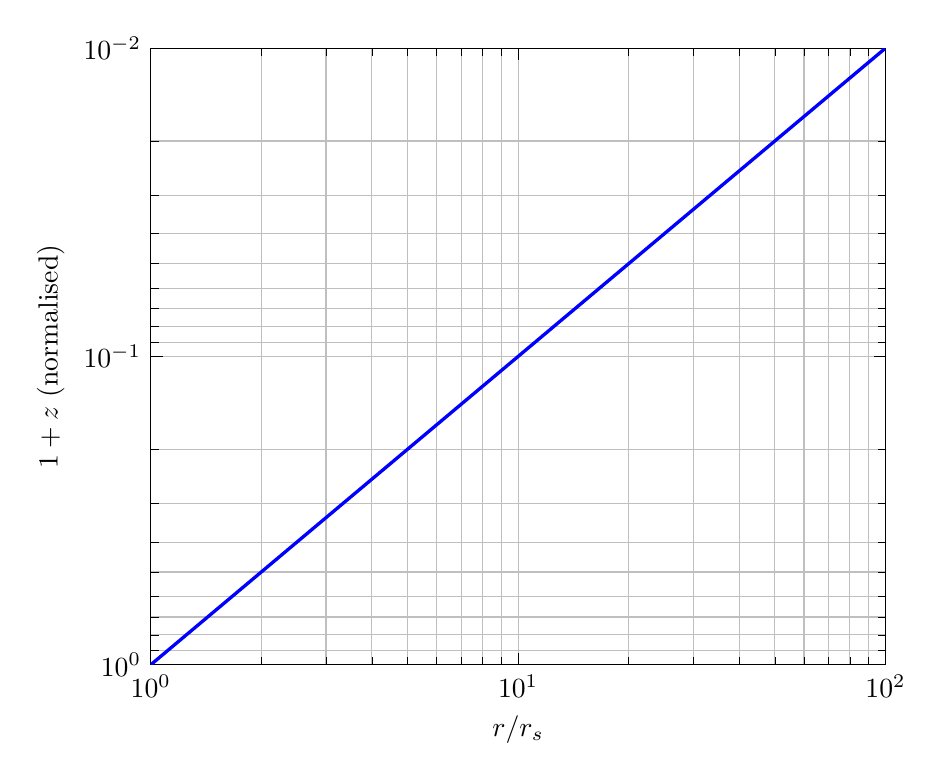
\begin{tikzpicture}
  \begin{axis}[
      width=0.9\textwidth,
      xlabel={$r/r_s$},
      ylabel={$1+z$ (normalised)},
      xmode=log, ymode=log,
      y dir=reverse,           % red-shift decreases with distance
      xmin=1, xmax=100,
      ymin=0.01, ymax=1,
      grid=both,
      tick style={black}]
    \addplot[very thick,blue,domain=1:100,samples=200] {1/x};
  \end{axis}
  \end{tikzpicture}
  %-------------------------------------------------------------
  \caption{$1/r$ gravitational red-shift around a $10^{9}M_{\odot}$ SMBH.}
  \label{fig:GravRedshift}
\end{figure}
